\chapter{Literature Review and My Niche}
\color{red}

To cite references, add BibTex fields into the \verb|biblio.bib| file in the main directory. In the text, use the \verb|\cite{}| command. For example, I used a design of experiments \citep{wu2011experiments} in studying the orientation of solar thermal collectors \citep{duffie2020solar} that collect total horizontal radiation \citep{hottel1976simple} and compared to the performance of focusing thermal collectors \citep{stine2001power}. 
If you find undefined references, make sure you have separately run the bibtex engine. In VS Code, you can do this by typing \verb|CTRL+SHIFT+P| and searching for ``latex recipe,'' then select \verb|pdflatex -> bibtex -> pdflatex x2|.

We illustrate use of graphics with an inline (standard) image in Figure~\ref{fig:1} and the same image with text wrapping in Figure~\ref{fig:2} on page~\pageref{fig:2}. 

\begin{figure}[htbp]
    \centering
    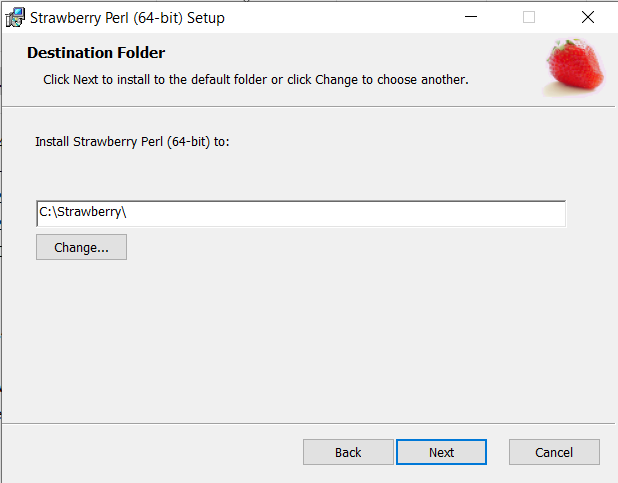
\includegraphics[width=0.5\linewidth]{image_001.png}
    \caption{A figure from the webpage}
    \label{fig:1}
\end{figure}

\color{black}

\lipsum[30-31]


\begin{wrapfigure}{L}{0.5\textwidth}  %l, r, L, R
    \centering
    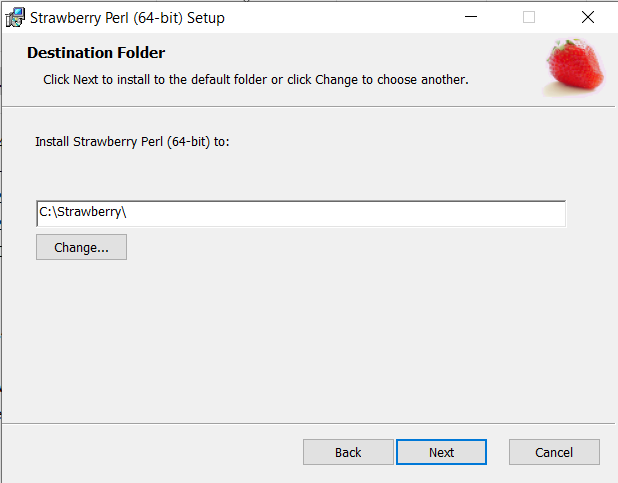
\includegraphics[width=\linewidth]{image_001.png}
    \caption{A figure is added with text wrapped.}
    \label{fig:2}
    \vspace{-2ex}
\end{wrapfigure}


\lipsum[32-33]
